\documentclass[12pt]{article}
\usepackage[utf8]{inputenc}
\usepackage{graphicx}
\usepackage[a4paper,width=150mm,top=25mm,bottom=25mm]{geometry}

\title{

\\
{COS 301 User Manual}
}



\author{Ctrl Alt Defeat}

\begin{document}

\begin{titlepage}
    \centering



    \vspace{2cm}
    \hrulefill\\
    \vspace{1cm}
    {\Huge\bfseries SRS Documentation v3.0}

    \vspace{1cm}

    {\Large Software Requirements Specification Document for\\Domain Pulse}\\
    \vspace{1cm}
    \hrulefill\\

    \vfill

    {\large Ctrl Alt Defeat}

    \vspace{1cm}

    {\large 2023/07/31}\\
    %    \vspace{1cm}
    %    \vspace{1cm}
    %    
\includegraphics[width=10cm]{../../Images/dpLogo.png}
    %    \vspace{1cm}\\
    %    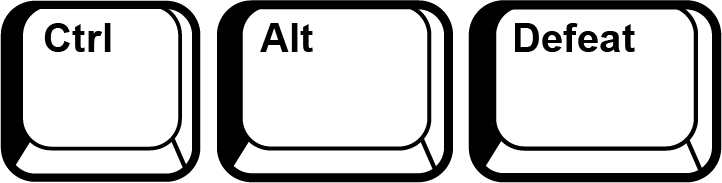
\includegraphics[width=6cm]{../../Images/cadLogo.png}

\end{titlepage}



\tableofcontents

\newpage



\section{Introduction}
\subsection{What is Domain Pulse?}
\begin{itemize}
    \item First we need to understand what Sentiment analysis is , Sentiment analysis is the process of computationally identifying and categorizing opinions expressed in a piece of text, especially in order to determine whether the writer's attitude towards a particular topic, product, etc. is positive, negative, or neutral. Now in this being said we introduce Domain Pulse.
    \item Domain pulse is the ultimate sentiment analysis platform. It gathers and analyses online opinions about any domain, be it a business, a person, or more. With stunning visuals and easy-to-understand statistics, Domain Pulse helps you understand the online presence and sentiment for any domain.
    \item Domain Pulse presents the results in a visually stunning and easy-to-understand
    format. Our wide range of visualisations bring statistics to life, which make it a breeze
    to grasp the online presence and sentiment for any domain. Take control of
    understanding public opinion like never before with Domain Pulse.
\end{itemize}
\subsection{Objectives of Domain Pulse}
\begin{itemize}
    \item The main objective of Domain Pulse is to provide a platform for users to analyse and gain valuable insight into the sentiment of any domain.
\end{itemize}
\newpage
\section{General access to the app}
\subsection{Logging into the app}
\begin{itemize}
    \item Simply add your email/username with which you registered with and your password and click on the blue 'login' button.
    \item Alternatively you can login with your Google account by clicking on the 'Sign in with Google' button.
    \item If you have forgotten your password, click on the 'Forgot Password?' link and follow the instructions.
    \item If you do not have an account, click on the 'Dont have an account?' link and register for an account using your chosen details.
\end{itemize}
\subsection{Registering for an account}
\begin{itemize}
    \item To register for an account the following information will be required:
    \begin{itemize}
        \item Username
        \item Email address
        \item Password
        \item Confirmation of password
    \end{itemize}
    \item Please enter the required information specified above in the relevant fields and click on the blue 'Register' button.
    \item If you already have an account , click on the 'Already have an account?' link and login with your registered details.
\end{itemize}
\newpage
\section{Dashboard}
\subsection{General overview}
\begin{itemize}
    \item The dashboard is the first page you will see when you log into the app.
    \item The dashboard will be the primary interactive page between the user and the app.
    \item A quick overview of the dashboard is as follows:
    \begin{itemize}
        \item On the left hand side of the page you will see a blue side bar 
        \item On the top of the page you will see the list of sources for chosen domain
        \item On the top right of the page are the actions that can be performed on certain components on the dashboard or the entire dashboard
        \item The center console of the page is where the insights and statistics will be displayed 
        \item On the bottom left you will see all the relevant graphs and charts displaying the statistics of the chosen source 
        \item On the bottom right of the page is sample data
    \end{itemize}
    \item A more detailed explanation of the dashboard will be given in the following sections
\end{itemize}

\section{In-depth dashboard overview}
\subsection{Adding a Domain}
\begin{itemize}
    \item To add a domain expand the sidebar and while the side bar is expanded , click on the 'add a domain' button
    \item The add Domain modal will appear , enter a domain name of your choice in the field , a description of your chosen domain and a chosen image for your domain 
    \item Domains will act as a 'folder' for your sources , so you can group sources together about a specific domain
\end{itemize}
\subsection{Removing a domain}
\begin{itemize}
    \item To remove a domain expand the sidebar and while the side bar is expanded , click on the 'bin' button , this will remove the specified domain after confirmation from the user.
\end{itemize}
\subsection{Editing a domain}
\begin{itemize}
    \item To edit a domain expand the sidebar and while the side bar is expanded , click on the 'edit' button , this will allow you to edit the name,description and image of the specified domain.
\end{itemize}
\subsection{Adding a source}
Navigate to the Select source bar at the top of the page:
\begin{itemize}
    \item This is where you can select sources for a chosen domain 
    \item Click on the blue 'plus' button to begin adding a source(show the plus button)
    \item Once the plus button is clicked , a modal will appear where you can add a source by entering the source name , chosing a source type(tested with Google reviews,Youtube and Tripadvisor) and entering the source URL which is a link from the repective source type for example a link from youtube and a link from the Tripadvisor website.Once you have entered the relevant information , click on the blue 'Confirm' button to add the source to the chosen domain(show the modal)
\end{itemize}
\subsection{Removing a source}
\begin{itemize}
    \item To remove a source , click on the source you would like to remove and click on the red bin button on the right hand side of the page , the source will be removed after confirmation from the user
\end{itemize}
\subsection{Refreshing a source or entire domain}
\begin{itemize}
    \item To refresh the data of a source or entire domain , click on the green refresh button on the right hand side of the page
\end{itemize}
\subsection{Editing a source}
\begin{itemize}
    \item To edit a source , click on the source you would like to edit and click on the yellow edit button on the right hand side of the page , an edit source modal will allow you to edit the source name , source type and source URL of a chosen source. Once you have edited the relevant information , click on the blue 'Confirm' button to save the changes
\end{itemize}
\subsection{Toggling a theme}
\begin{itemize}
    \item To toggle a theme , click on the profile icon at the bottom of the sidebar , a profile modal will appear , click on the 'Toggle Theme' button to toggle between a light and dark theme
\end{itemize}
\subsection{Log out}
\begin{itemize}
    \item To log out , click on the profile icon at the bottom of the sidebar , a profile modal will appear , click on the 'Log out' button to log out of the app
\end{itemize}
\subsection{Change password}
\begin{itemize}
    \item To change your password , click on the profile icon at the bottom of the sidebar , a profile modal will appear , click on the 'Change Password' button to change your password ... another pop up modal will appear where you will be required to enter your current password and your new password , once you have entered the relevant information , click on the blue 'Confirm' button to save the changes
\end{itemize}
\subsection{Delete account}
\begin{itemize}
    \item To delete your account , click on the profile icon at the bottom of the sidebar , a profile modal will appear , click on the 'Delete Account' button and you will be required to enter your password to confirm the deletion of your account
\end{itemize}
\subsection{Update profile picture}
\begin{itemize}
    \item To update your profile picture click on the profile icon at the bottom of the sidebar and a profile modal will appear , click on the Profile picture itself to update your profile picture and then click the 'Confirm' button to save the changes
\end{itemize}

\newpage



\subsection{Explanation of entire dashboard}
\begin{itemize}
    \item Blue sidebar on the left hand side of the page:
    \begin{itemize}
        \item This is where you will be able to choose the domain you wish to generate statistics for (show the different domains in a photo)
        \item This is where you can group sources together about a specific domain
        \item When the sidear is expanded , you can edit or remove a domain of your choice as specified in section 
        \item At the bottom of the sidebar you can view and manage your profile which will be discussed further in the following section(show the profile modal before it is clicked on)
    \end{itemize}
    \item Profile modal at the bottom of the expanded sidebar:
    \begin{itemize}
        \item This is where you can view your profile information and perform relevant actions regarding your preferences and profile settings(have a picture of the expanded profile modal and show all buttons below)
        \item The theme can be toggled from a light theme to a dark theme or vice versa by clicking on the 'Toggle Theme' button
        \item You will be logged out of the app if you click on the 'Logout' button
        \item You can change your password by clicking on the 'Change Password' button
        \begin{itemize}
            \item Once you have clicked on the 'Change Password' button , a modal will appear where you can enter your current password and your new password.Once you have entered the relevant information , click on the blue 'Confirm' button to change your password(show the modal)
        \end{itemize}
        \item You can delete your account by clicking on the 'Delete Account' button
        \item If you would like to return to the dashboard , click the back arrow in the top left corner of the modal
    \end{itemize}
    \item Select source bar at the top of the page:
    \begin{itemize}
        \item This is where you can select sources for a chosen domain 
        \item Click on the blue 'plus' button to begin adding a source(show the plus button)
        \item Once the plus button is clicked , a modal will appear where you can add a source by entering the source name , chosing a source type(tested with Google reviews,Youtube and Tripadvisor) and entering the source URL.Once you have entered the relevant information , click on the blue 'Confirm' button to add the source to the chosen domain(show the modal)
    \end{itemize}
    \item Actions on the top right of the page:
    \begin{itemize}
        \item The green refresh arrow will refresh the sources data to check if any new relevant information has been added to a source and update the statistics and insights(show button)
        \item The yellow edit button will allow you to edit a source with an edit source modal(show button before and after click)
        \begin{itemize}
            \item The edit source modal will allow you to edit the source name , source type and source URL of a chosen source. Once you have edited the relevant information , click on the blue 'Confirm' button to save the changes(show modal)
        \end{itemize}
        \item The red delete button will delete the highlighted source from the chosen domain(show button)
        \item inspect button???????????????????????
    \end{itemize}
    \item Center console of the page:
    \begin{itemize}
        \item This is where the insights and statistics will be displayed
        \item Starting on the left hand side of the center console:
        \begin{itemize}
            \item The first Statistic displayed is the overall score which is the ratio of positive and negative sentiment of a chosen domain , the higher the score the more positive the sentiment and vice versa
            \item Next is the amount of positive,negative and neutral sentiment of a chosen domain which are represented in percentages, the higher the percentage the more that sentiment is present in the chosen domain.
            \item The Emotion block of the center console is the most prevalent emotion of a chosen domain , the emotions detectable are anger,disgust,fear,joy,neutral sadness and surprise.
            \item The toxicity block analysis aims to assess the level of harmfulness or offensiveness in the text and classify it accordingly.
            \item The analysed block is the amount of sentiment that has been analysed in a chosen domain.
            \item Finally the range block is the timeframe in which the data has been collected to calculate the statistics and insights.
        \end{itemize}
    \end{itemize}
    \item Graphs and charts on the bottom left of the page:
    \begin{itemize}
        \item The graphs shown are graphical representations of the statistics and insights shown in the center console of the page.
        \item clicking on the arrows on the left and right of the graphs will allow you to view the graphs of the previous and next statistic respectively.
    \end{itemize}
    \item Sample data on the bottom right of the page:
    \begin{itemize}
        \item This is where you can view sample data of a chosen domain.
        \item To view the sample data just scroll up or down to view the data.
    \end{itemize}
\end{itemize}
\end{document}
